\documentclass[a4paper]{article}
\usepackage[utf8]{inputenc}
\usepackage[russian]{babel}
\usepackage{float}
\usepackage{graphicx}
\usepackage{amsmath}
\usepackage{amssymb}
\usepackage{amsthm}
\usepackage[unicode, pdfborder = {0 0 0}, colorlinks, linkcolor = black]{hyperref}


\parindent = 7mm
\oddsidemargin = 5mm
\topmargin = -10mm
\textheight = 240mm
\textwidth = 165mm
\linespread{1.5}


\renewcommand{\small}{\fontsize{12}{14.5pt}\selectfont}
\renewcommand{\normalsize}{\fontsize{14}{16pt}\selectfont}
\renewcommand{\large}{\fontsize{17}{20pt}\selectfont}
\renewcommand{\Large}{\fontsize{20}{25pt}\selectfont}
\renewcommand{\LARGE}{\fontsize{25}{30pt}\selectfont}
\renewcommand\qedsymbol{$\blacksquare$}

\newtheorem{theorem}{Теорема}[section]
\theoremstyle{definition}
\newtheorem{statement}{Утверждение}[section]
\newtheorem{definition}{Определение}[section]
\newtheorem*{example}{Пример}

\newenvironment{Proof}
    {{\bf \flushleft{Доказательство.} \\}}
    {\hfill$\scriptstyle\blacksquare$}


\begin{document}
\normalsize

    \thispagestyle{empty}
    \begin{titlepage}
    \begin{center}


    \vfill
    МИНОБРНАУКИ РОССИИ\\
    \vspace*{0.3cm}
    Федеральное государственное автономное образовательное\\
    учреждение высшего образования\\
    «Южный федеральный университет»\\
    \vspace*{0.3cm}
    Институт математики, механики и компьютерных наук им.\\
    И.И.Воровича\\
    Кафедра алгебры и дискретной математики
    \vfill


    \bigskip


    {\large\bf Ковалев~Никита~Евгеньевич}
    \vfill
    {\large\bf ВОССТАНОВЛЕНИЕ ИЗОБРАЖЕНИЙ\\
               С ВЫРОЖДЕННЫМ СМАЗОМ}

\fontsize{14}{16pt}\selectfont

    \vfill
    ВЫПУСКНАЯ КВАЛИФИКАЦИОННАЯ\\ РАБОТА БАКАЛАВРА\\
    по направлению 01.03.02 — Прикладная математика и информатика
    \vfill

    {\bf Научный руководитель~---\\
         доц., к.ф.-м.н. Козак Анатолий Всеволодович}



    \vfill

    \end{center}

    \bigskip

    \begin{center}
        Ростов-на-Дону~---~2017
    \end{center}

    \end{titlepage}

%-------------------------------------
    \tableofcontents
    \newpage
%-------------------------------------

    \begin{center}
        \section*{Введение}
        \addcontentsline{toc}{section}{Введение}
    \end{center}


    В данной работе рассматривается явление горизонтального циклического смаза. Само являение возникает при съемке местности с помощью вращающейся камеры при создании панорманых снимков. При возникновении этого явления смазанное изображение содержит большое количество искаженной (потерянной) информации, соответственно, появляется необходимость восстановить эти данные.


    Поскольку задача актуальна для таких областей, как военная разведка, картография, геодезия, моделирование объектов местности и других, то отснять материал заново зачастую невозможно. В силу этой специфики задача восстановления искаженных снимков приобретает наиважнейший характер.


    Введем некоторые обозначения и базовые понятия, которые будут использоваться в дальнейшем.
\vspace*{0.3cm}


    \begin{definition}
    \label{blur matrix}
	\emph{Матрицей горизонтального циклического смаза} (далее - \emph{матрицей смаза}) на $k$ пикселей называется матрица $C(n, k) \in M_n$ вида
    $$
    C(n, k) = \frac{1}{k}\begin{pmatrix}
          \overbrace{1 \hspace*{2mm} \ldots \hspace*{2mm} 1 \hspace*{2mm} 1}^{k} \hspace*{2mm} 0 \hspace*{2mm} \ldots \hspace*{2mm} 0 \\
          0 \hspace*{2mm} 1 \hspace*{2mm} \ldots \hspace*{2mm} 1 \hspace*{2mm} 1 \hspace*{2mm} \ldots \hspace*{2mm} 0 \\
          \ldots \hspace*{2mm} \ddots \hspace*{2mm} \ldots \hspace*{2mm} \ddots \hspace*{2mm} \ldots \\
          1 \hspace*{2mm} \ldots \hspace*{2mm} 0 \hspace*{2mm} 1 \hspace*{2mm} 1 \hspace*{2mm} \ldots \hspace*{2mm} 1 \\
          \ldots \hspace*{2mm} \ddots \hspace*{2mm} \ldots \hspace*{2mm} \ddots \hspace*{2mm} \ldots\\
          \underbrace{1 \hspace*{2mm} \ldots \hspace*{2mm} 1}_{k-1} \hspace*{2mm} 0 \hspace*{2mm} 0 \hspace*{2mm} \ldots \hspace*{2mm} 1
        \end{pmatrix}
    $$
    \end{definition}


    В дальнейшем будем отождествлять понятие матрицы смаза и обозначения $C(n, k)$ и просто $C$ (если параметры $n$ и $k$ ясны из контекста).
\vspace{0.3cm}


    \begin{definition}
    \label{blur}
	\emph{Горизонтальным циклическим смазом} (далее - \emph{смазом}) будем называть умножение изображения на соответствующую матрицу смаза справа.
    \end{definition}


    \begin{statement}[об обратимости матрицы смаза]
    \label{inverse}
	Матрица смаза обратима тогда и только тогда, когда НОД$(n, k) = 1$.
    \end{statement}


    Следствием \ref{inverse} является, среди прочего, большее количество изображений с вырожденным смазом, нежели с невырожденным, что лишний раз подтверждает актуальность поставленной задачи.


    \begin{example}
    Приведем пример изображения и его смазанную копии.

\begin{minipage}{70mm}
    \begin{figure}[H]
            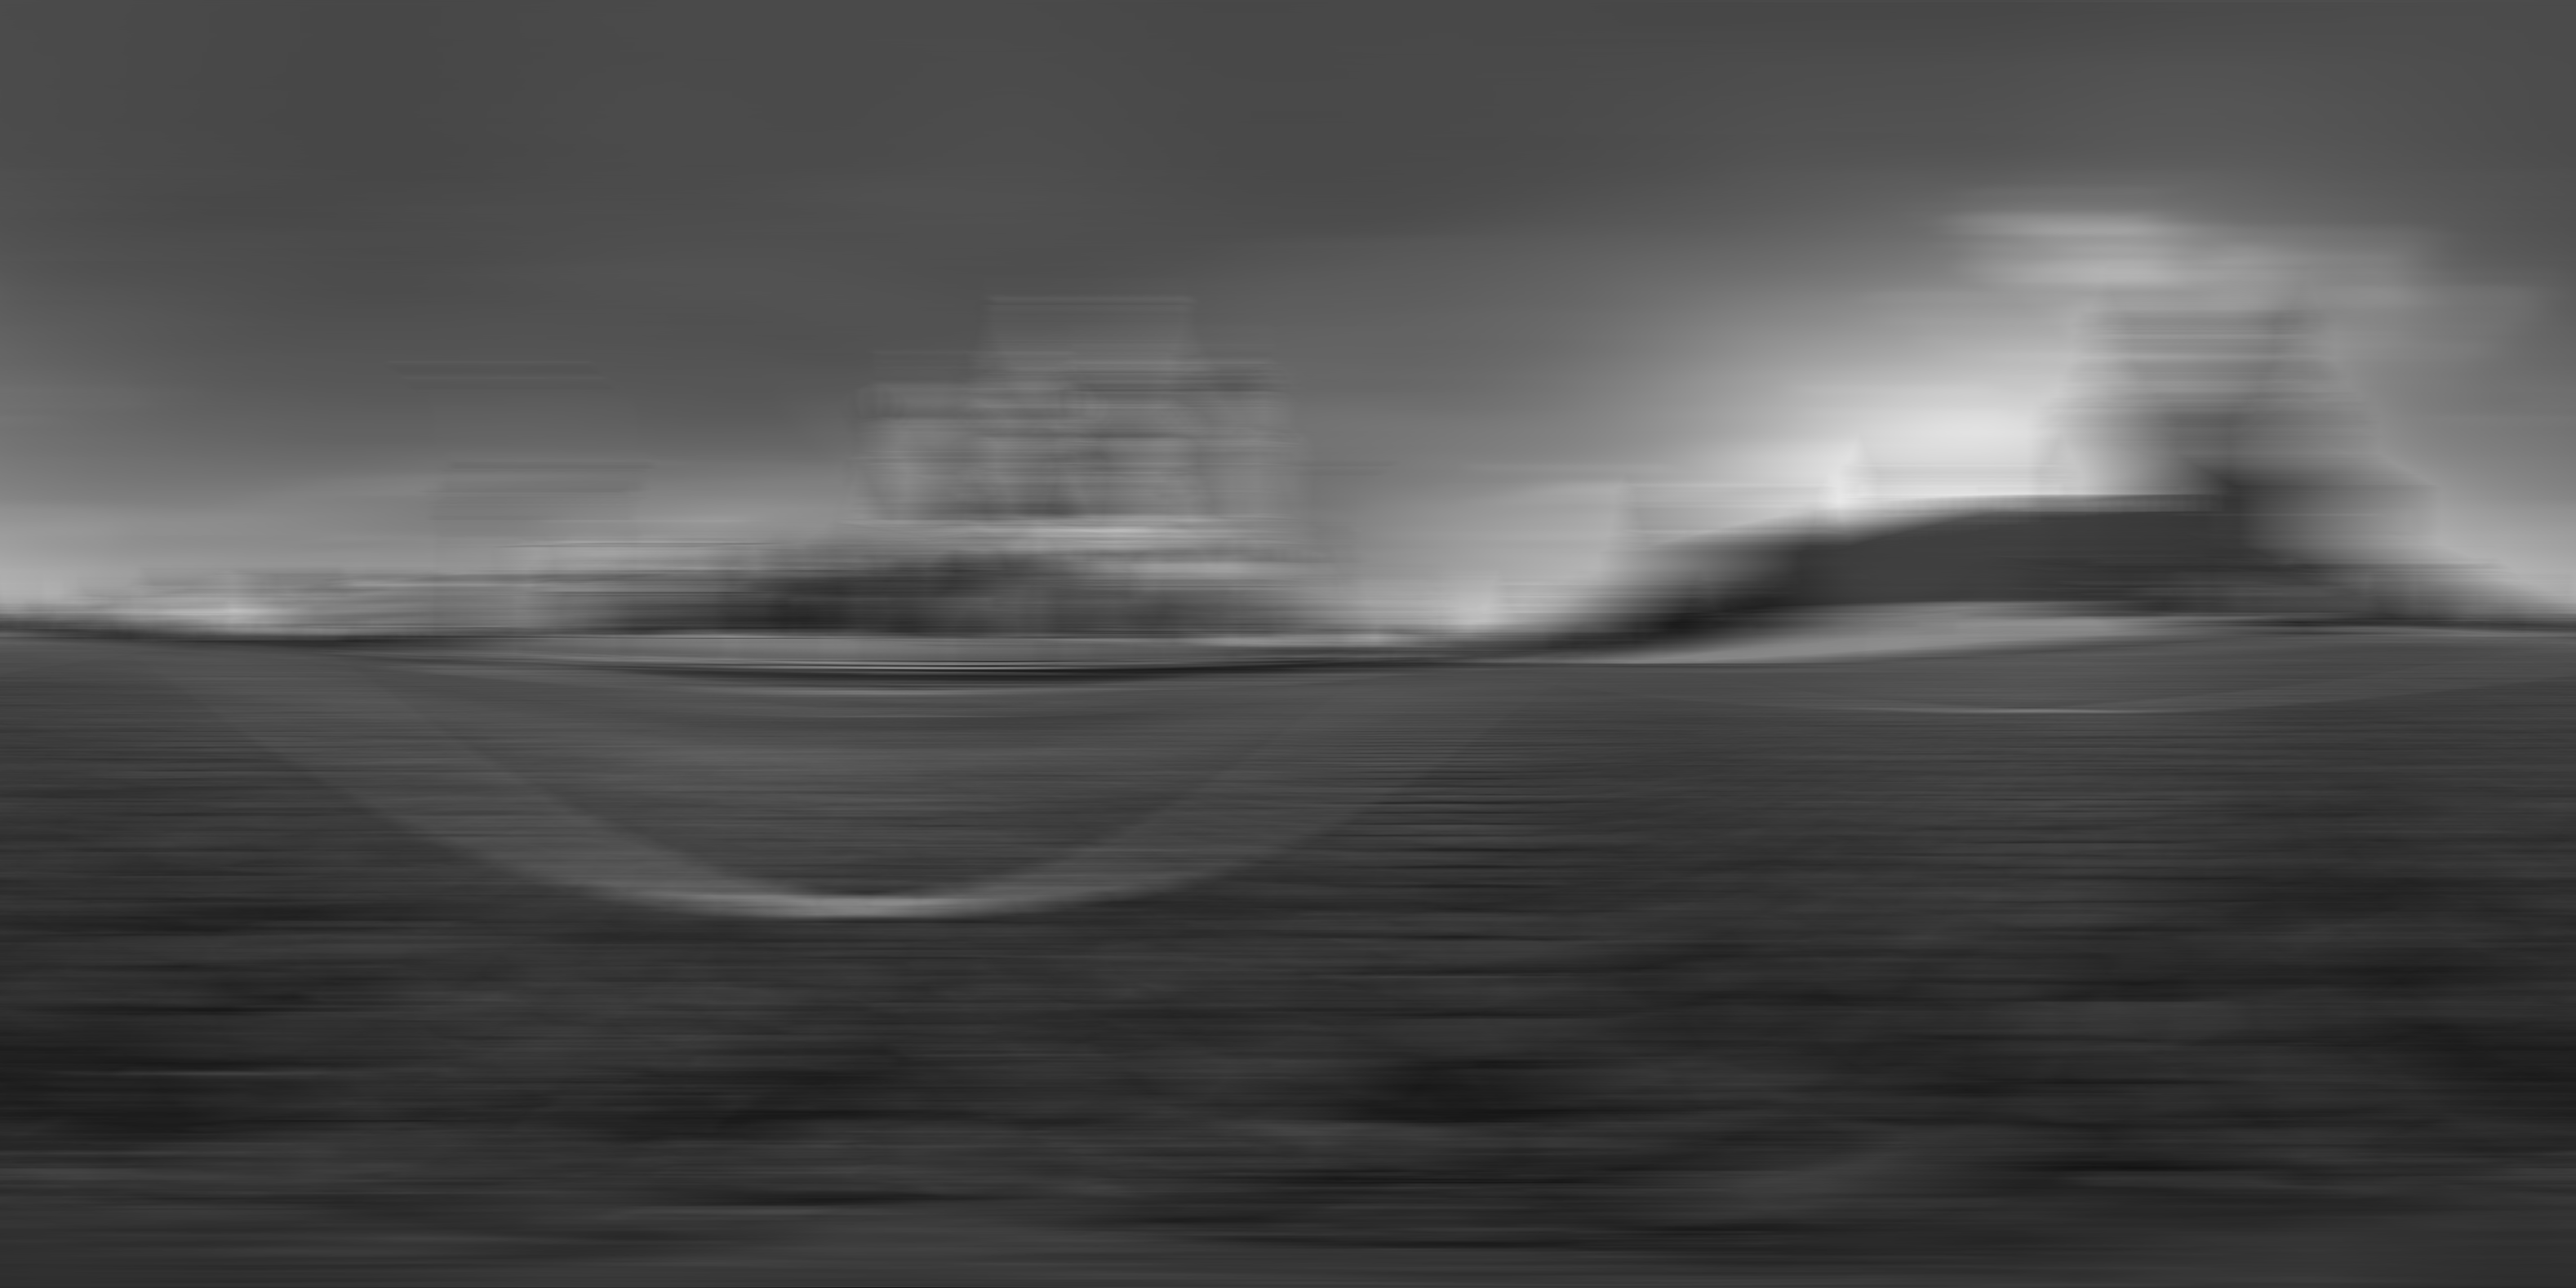
\includegraphics[scale=0.07]{D:/Diploma/Pictures/fig1.png}
            \label{Fig1}
            \caption[Смаз при $k$ = 248]{Смаз при $k$ = 248}
        \end{figure}
\end{minipage}
\hfill
\begin{minipage}{70mm}
  \begin{figure}[H]
            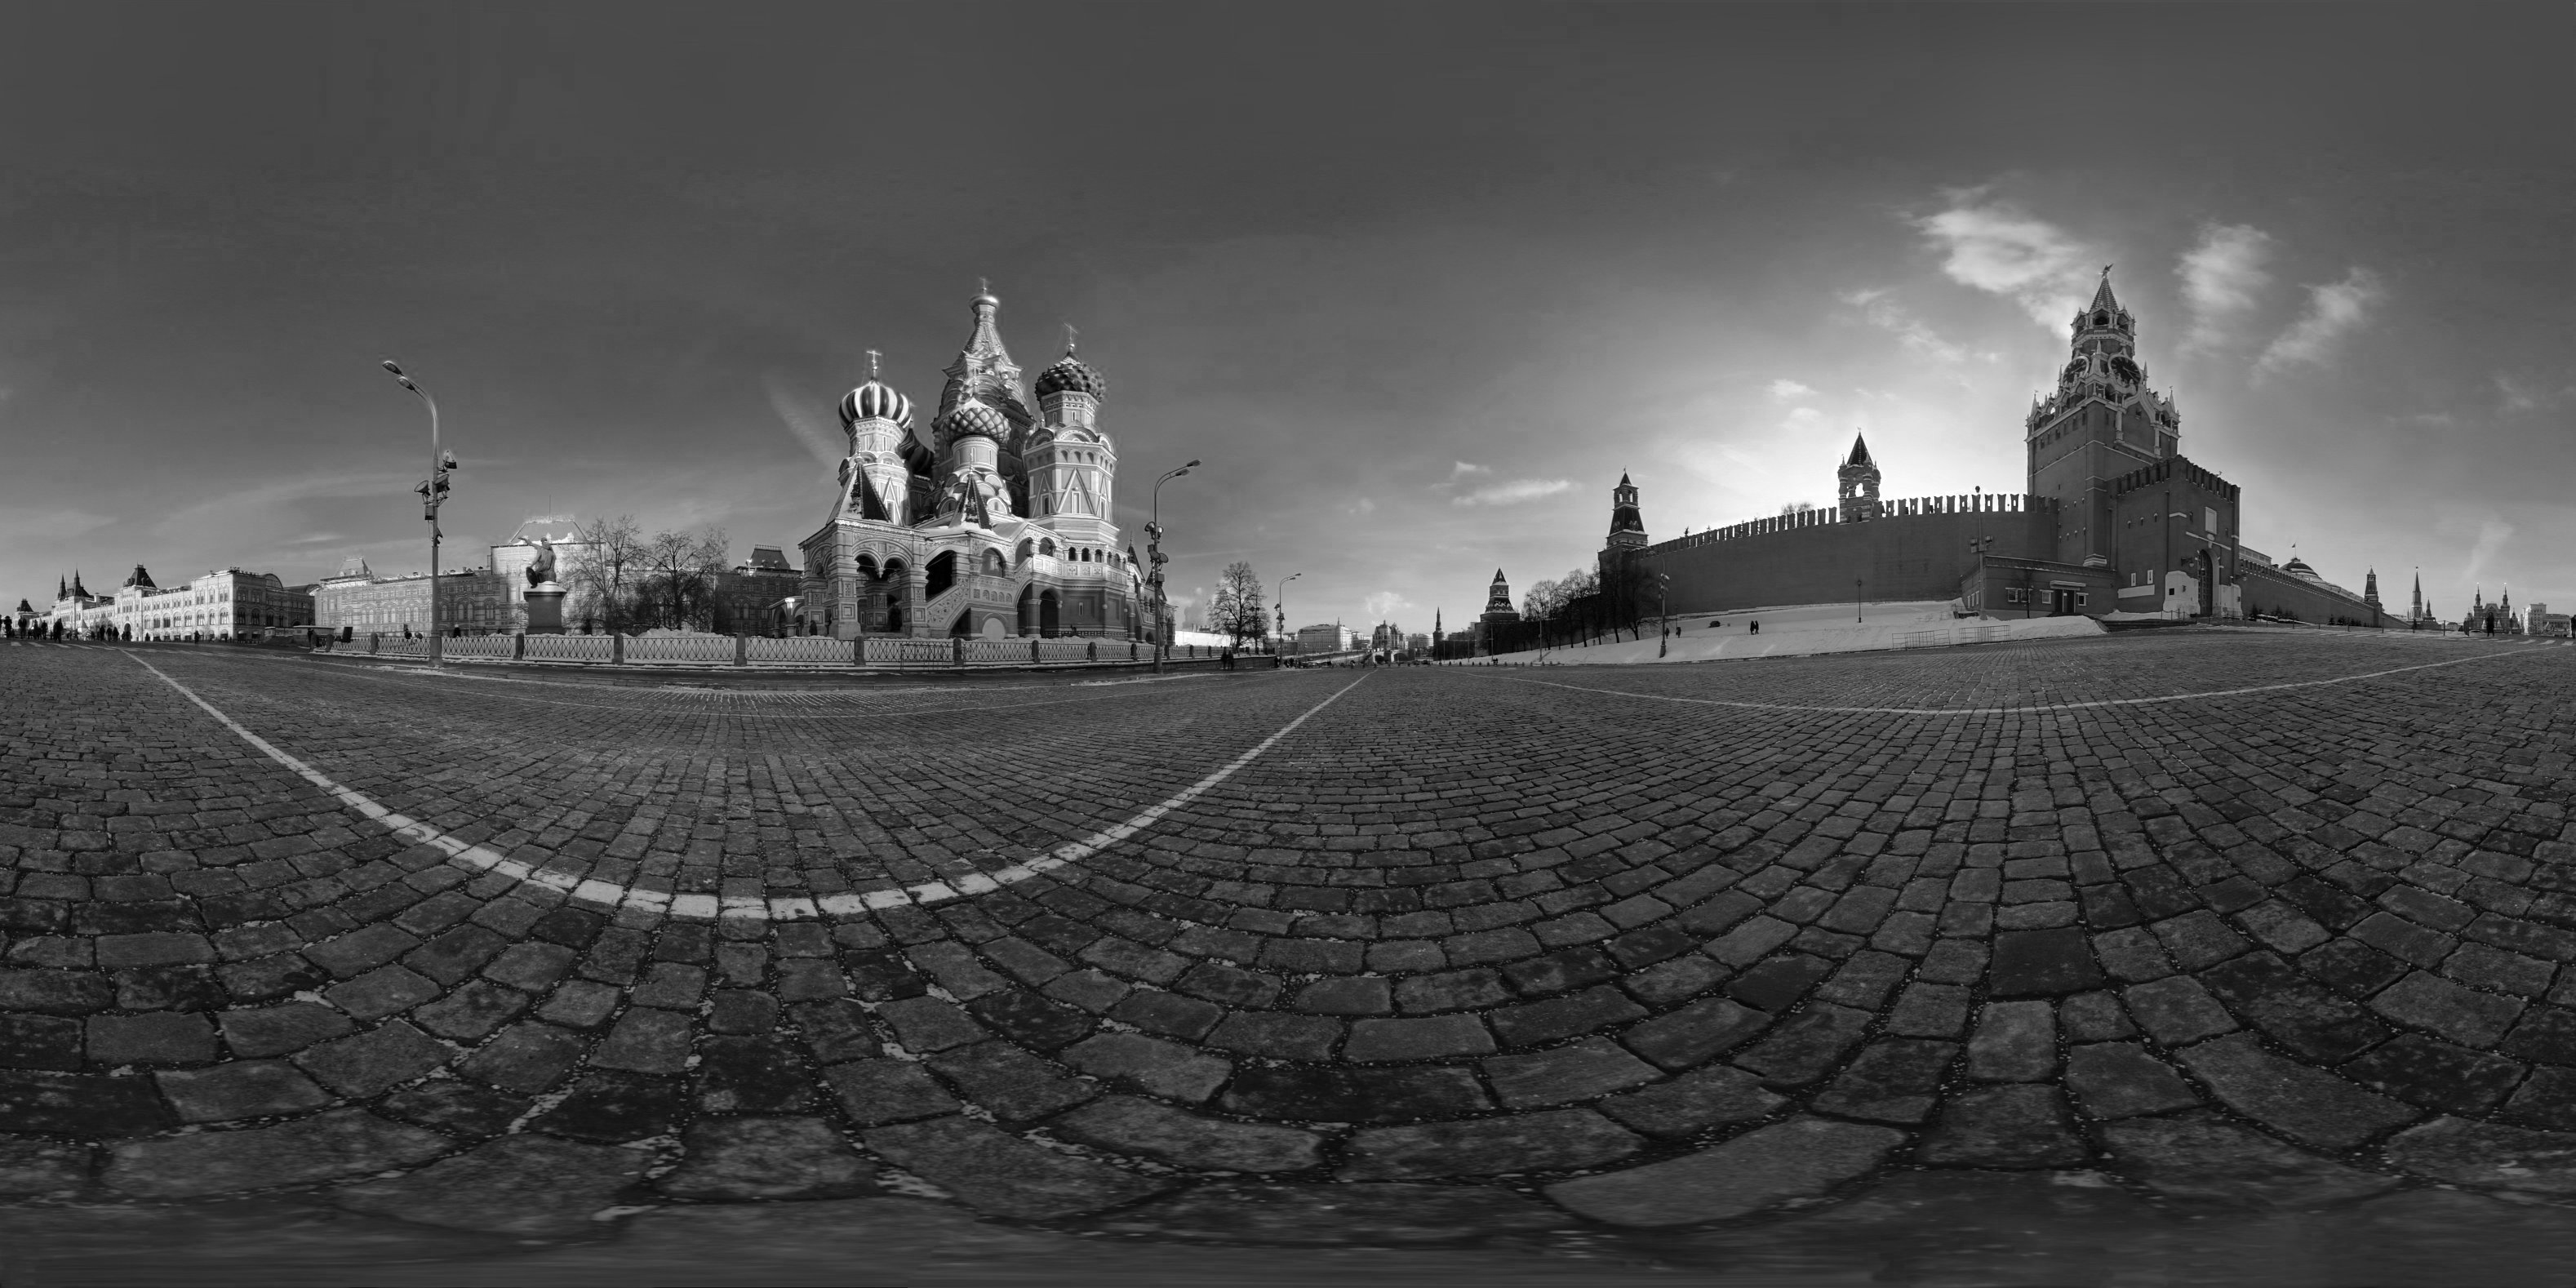
\includegraphics[scale=0.07]{D:/Diploma/Pictures/fig2.png}
            \label{Fig2}
            \caption[Исходное изображение]{Исходное изображение}
        \end{figure}
\end{minipage}
\hfill

    \end{example}

%--------------------------------------
    \newpage


    \begin{center}
        \section*{Метод предобработки в случае большого числа смаза}
        \addcontentsline{toc}{section}{Метод предобработки в случае большого числа смаза}
    \end{center}


    В первом параграфе пойдет речь о методе, который эффективен только для восстановления 16-битных изображений, поскольку данный подход использует обычное восстановление для невырожденного случая, а оно эффективно только для 16-битных изображений. В силу этих ограничений метод интересен не столько своей практической пригодностью, сколько подходом, который, возможно, применим в комбинации с лучшим методом восстановления.


    Подход заключается в следующем: в случае вырожденного смаза имеем $d =$ НОД$(n, k) > 1$, где $k$ - число смаза, $n$ - ширина изображения в пискелях. Тогда поделим исходное изображение $I$ на $d$ подизображений, каждое из которых содержит $i$-й столбец и далее каждый столбец, на $d$ правее предыдущего выбранного. В итоге получим последовательность $\{I_j\}_{j=1}^{d}$, каждое изображение которой содержит $\frac{n}{d}$ пискелей в ширину. Однако, каждое из этих изображений будет содержать смаз уже не на $k$, а на $\frac{k}{d}$, и, так как $d =$ НОД$(n, k)$, то НОД$(\frac{n}{d}, \frac{k}{d}) = 1$, следовательно, смаз невырожденный. Восстанавливая $I_j$ и объединяя их по тому же принципу, по какому происходило и разделение, мы получим изображение, содержащее смаз на $d$ пикселей. Объясняется это тем, что каждая из восстановленных картинок предоставляет $\frac{1}{d}$ информации от необходимой, но информация разных частей не является уникальной - все они несут примерно одну и ту же информацию. Это подтверждается экспериментально на реальных примерах.



\end{document}